\documentclass{beamer}
\usetheme{Boadilla}
\usecolortheme{sidebartab}

\usepackage{hyperref}
\usepackage{showexpl} 
\usepackage{graphicx}
\usepackage{color}
\usepackage{siunitx}
\usepackage[version=3]{mhchem}
\usepackage{chemfig}
\usepackage{changes}

\lstloadlanguages{[LaTeX]Tex} 
\lstset{% 
     basicstyle=\ttfamily\large, 
     commentstyle=\itshape\ttfamily, 
     showspaces=false, 
     showstringspaces=false, 
     breaklines=true, 
     breakautoindent=false, 
     captionpos=t,
     explpreset={numbers=none},
     pos=b
} 

\title{Introduction to writing with LaTeX}
\author{Markus Stocker}
\date{May 12, 2017}

\begin{document}

% Ask who knows about LaTeX and who has already experimented with it
% Any expert users?
\maketitle

\begin{frame}
  \frametitle{Outline}
  
  \begin{itemize}
  \item Morning lecture
  \begin{itemize}
  \item What is \LaTeX
  \item Motivating \LaTeX 
  \item \LaTeX~software environment
  \item Basics of writing \LaTeX~documents
  \item BibTeX reference management
  \item Scientific documents with journal \LaTeX~templates
  \item \LaTeX~for slides and posters
  \item Collaborative writing and versioning of \LaTeX~documents
  \end{itemize}
  \item Afternoon hands-on
  \begin{itemize}
  \item Develop your \LaTeX~article
  \item Style your article with journal templates
  \item Revise your article tracking changes
  \item Create slides and a poster to present your work
  \item Collaborative writing with your co-authors
  \end{itemize}
  \end{itemize}
\end{frame}

\begin{frame}
  \frametitle{Schedule}
  
  \begin{center}
  \begin{tabular}{ll}
  10.00 - 11.30 & Lecture \\
  11.30 - 12.30 & \emph{Lunch} \\
  12.30 - 13.15 & Hands-on I \\
  13.15 - 13.30 & \emph{Break} \\
  13.30 - 14.15 & Hands-on II \\
  14.15 - 14.45 & \emph{Coffee break} \\
  14.45 - 15.30 & Hands-on III \\
  15.30 - 15.45 & \emph{Break} \\
  15.45 - 16.30 & Hands-on IV \\
  16.30 - 17.00 & Closing
  \end{tabular}
  \end{center}
\end{frame}

\begin{frame}
  \frametitle{About me}
  
  \begin{itemize}
  \item Postdoc with PANGAEA at MARUM
  \item PhD in environmental informatics at University of Eastern Finland
  \item MSc in informatics at University of Zurich
  \item MSc in environmental science at University of Eastern Finland \emph{(soon)}
  \item My history with \LaTeX~goes back to 2001 when ...
  \end{itemize}
\end{frame}

\begin{frame}
  \frametitle{What is \LaTeX}
  
  \begin{itemize}
  \item Document preparation system
  \item Authored by Leslie Lamport, first released in 1985
  \item Most often used for technical or scientific documents
  \item Separate presentation from content
  \item Worry less about style and more about content
  \item Write plain text rather than formatted text
  \item Leave document design to designers
  \item Free software
  \item Available for Windows, Mac OS, Linux, Online
  \end{itemize}
  
  \begin{flushright}
  \url{https://www.latex-project.org}
  \end{flushright}
\end{frame}


\begin{frame}[fragile]
  \frametitle{What is \LaTeX}
	
  \begin{itemize}
  \item \textbf{Markup tagging} is central to writing with \LaTeX
  \item Label parts of the document using tags, e.g. \lstinline!\textit{}!
  \item It is used to do things like
  \begin{itemize}
  \item Define document structure, e.g. chapters, sections
  \item Style text, e.g. italic, symbols, tables
  \item Cite, footnote, cross-reference, ...
  \end{itemize}
  \item Anyone familiar with HTML?
  \end{itemize}
\end{frame}

\frame[containsverbatim]{ 
  \frametitle{Markup tagging}
		
  \begin{LTXexample}
\textit{Example} 
markup 
\underline{tagging}
  \end{LTXexample}
}

\frame[containsverbatim]{ 
  \frametitle{Markup tagging}
	
  \begin{LTXexample}
\begin{itemize}
\item Eggs
\item Milk
\item Cheese
\item Carrots
\end{itemize}
  \end{LTXexample}
}

\frame[containsverbatim]{ 
  \frametitle{Markup tagging}
	
  \begin{LTXexample}
$ E = mc^2 $
  \end{LTXexample}
}

\begin{frame}
  \frametitle{Why \LaTeX: Advantages}
  
  \begin{itemize}
    \item High typographic quality
    \item Excels at difficult typesetting tasks, e.g. mathematical text
    \item Makes things easy, e.g. citation, cross-reference, table of content
    \item Great engineering, fast and stable
    \item Even with long and complex documents
    \item No corrupt files, content loss, etc.
    \item Truly portable across systems
  \end{itemize}
\end{frame}

\begin{frame}
  \frametitle{Why \emph{not} \LaTeX: Disadvantages}
	
  \begin{itemize}
    \item Learning curve, somewhat difficult to learn
    \item Though, basics are \emph{really} easy
    \item Surely requires some time
    \item Not WYSIWYG
    \item More difficult in collaborative writing
    \item Less support for tracking changes
  \end{itemize}
\end{frame}

\begin{frame}
  \frametitle{Working with \LaTeX}
	
  \begin{itemize}
    \item You need a distribution
    \begin{itemize}
      \item Most likely TeX Live (\url{http://www.tug.org/texlive/})
      \item Or MiKTeX on Windows (\url{https://miktex.org/})
      \item Possibly MacTeX (\url{http://www.tug.org/mactex/})
    \end{itemize}
    \item Some kind of editor
    \item If you like Notepad, Vim, Emacs, ...
    \item Preferably,
    \begin{itemize}
      \item TeXstudio (\url{http://texstudio.org/})
      \item Texmaker (\url{http://www.xm1math.net/texmaker/})
      \item TeXnicCenter on Windows (\url{http://www.texniccenter.org/})
      \item TeXShop on Mac OS (\url{http://pages.uoregon.edu/koch/texshop/})
      \item Among others ...
    \end{itemize}
    \item Make use of packages, of which there are several thousands
  \end{itemize}
\end{frame}

\begin{frame}
  \frametitle{Working with \LaTeX}
  
  \begin{enumerate}
    \item Install distribution and editor
    \item Install required packages
    \item Write \LaTeX~document using editor
    \item Translate \LaTeX~document into PDF document
    \item Iterate over points (2) and 3-4 until done
  \end{enumerate}
\end{frame}

\begin{frame}
  \frametitle{TeXstudio}
  
  \begin{center}
    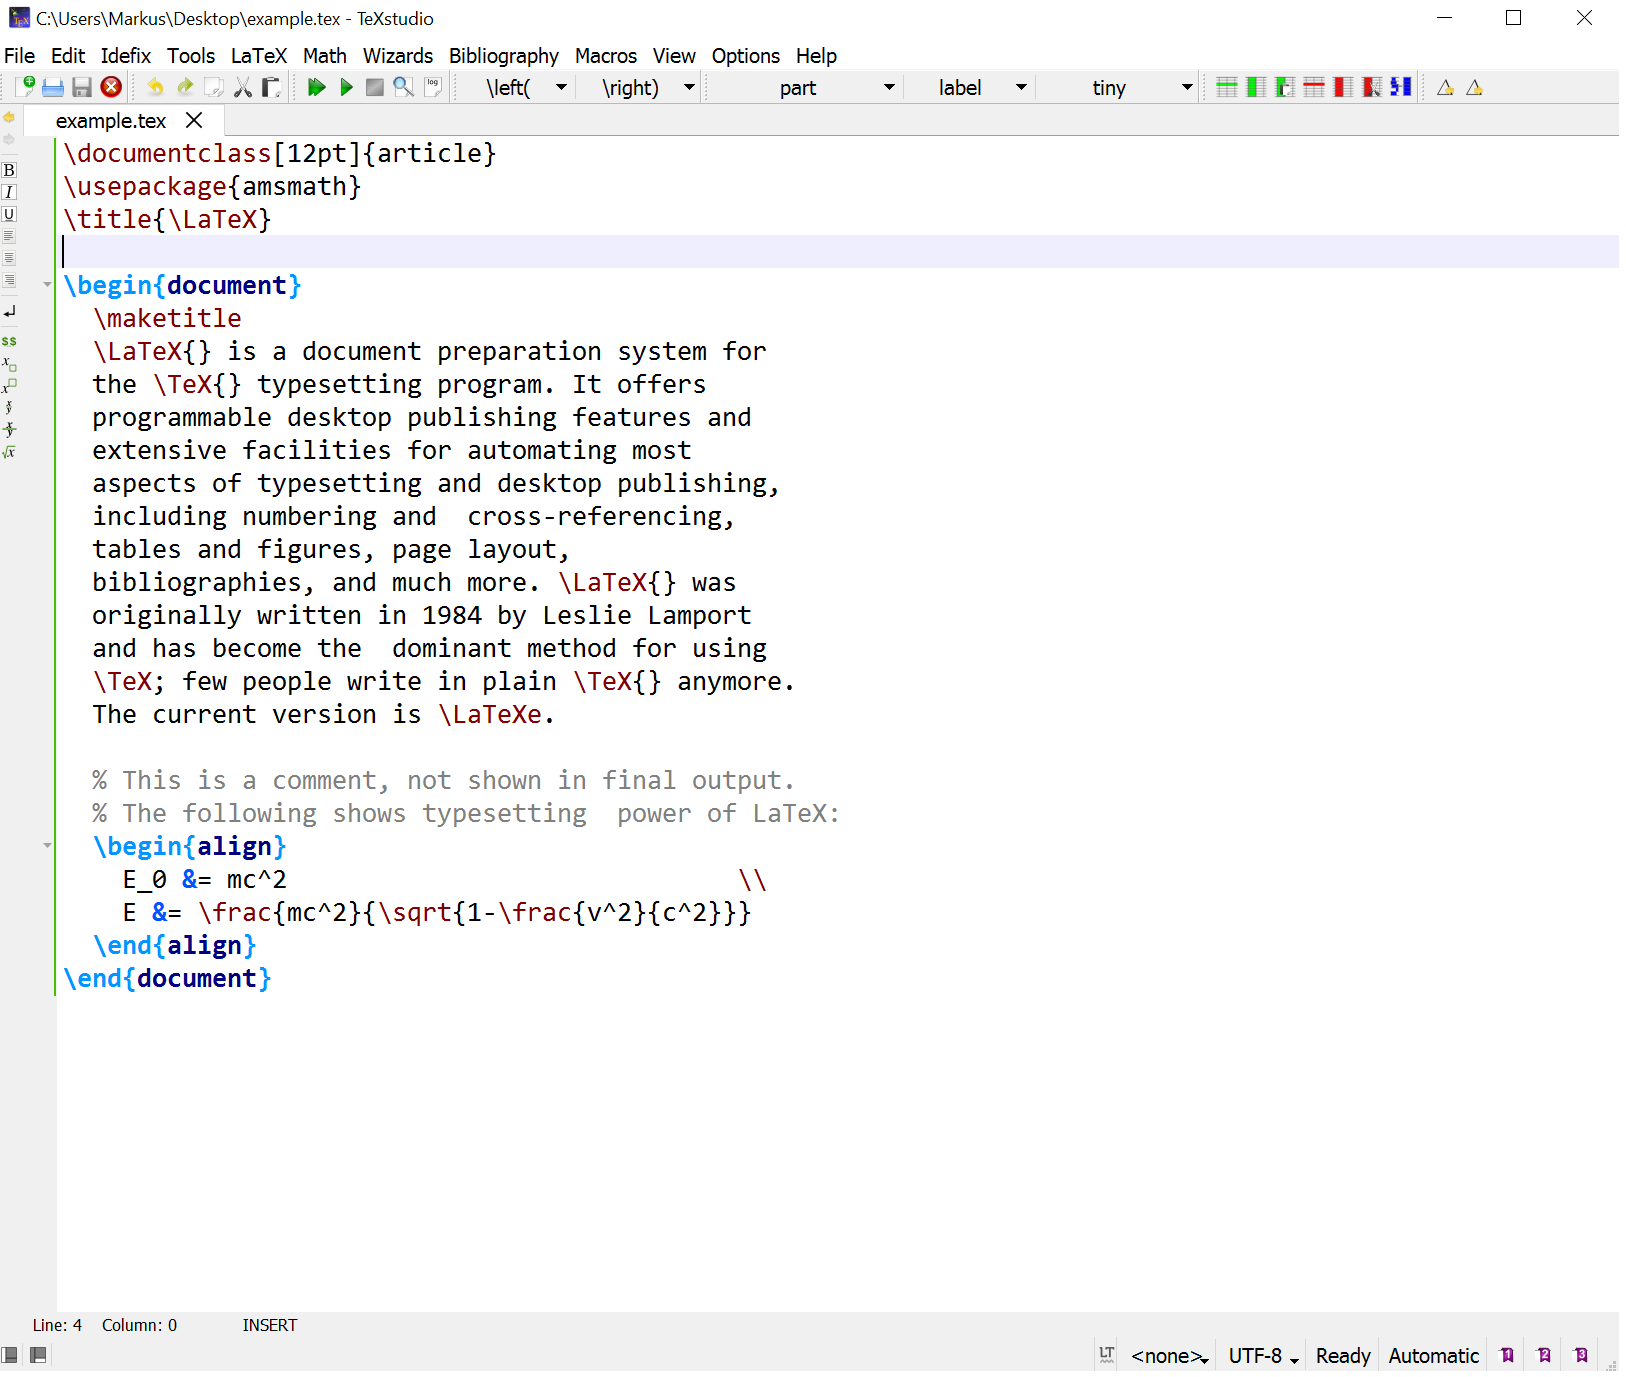
\includegraphics[height=0.8\textheight]{figures/texstudio.png}
  \end{center}
\end{frame}

\begin{frame}
  \frametitle{Writing \LaTeX~documents}
  
  \begin{itemize}
    \item Start with minimal document
    \item Develop it gradually by introducing new elements
    \item Structural elements, e.g. title, sections
    \item Style text, e.g. font size, italic, bold
    \item Mathematical and chemical formulae, quantities and units
    \item Tables, graphics and figures
    \item Cross-references, footnotes, and index
    \item Citation and reference list
    \item Table of contents, list of figures and tables
    \item Tracking changes
  \end{itemize}
\end{frame}

\frame[containsverbatim]{
  \frametitle{Minimal document}
 
  \begin{verbatim}
  \documentclass{article}
  
  \begin{document}
    Hello World.
  \end{document}
  \end{verbatim}
}

\begin{frame}
  \frametitle{Minimal document}
  
  \begin{center}
    
\includegraphics[width=0.3\textwidth]{figures/minimal.pdf}
  \end{center}
\end{frame}

\frame[containsverbatim]{
  \frametitle{Minimal document}
  
  \begin{verbatim}
  \documentclass{article}
  
  % I am a comment
  % This area is called the PREAMBLE
  % Used to load packages and configure your document
  
  \begin{document}
  
  % This is the BODY of the document
  % Document content goes here
  
  \end{document}
  \end{verbatim}
}

\frame[containsverbatim]{
  \frametitle{Article title}
  
  \begin{verbatim}
  \documentclass{article}
 
  \title{Shine On You Crazy Diamond}
  \author{Pink Floyd}
  \date{1975}
  
  \begin{document}
    \maketitle % Don't worry how it is displayed
               % It will look pretty good
  \end{document}
  \end{verbatim}
}

\begin{frame}
  \frametitle{Article title}
  
  \begin{center}
    
\includegraphics[width=0.8\textwidth]{figures/maketitle.pdf}
  \end{center}
\end{frame}


\frame[containsverbatim]{
  \frametitle{Article sections}
  
  \begin{verbatim}
  \documentclass{article}
  
  \title{Shine On You Crazy Diamond}
  \author{Pink Floyd}
  \date{1975}
  
  \begin{document}
    \maketitle
    
    \section{Introduction}
    \section{History}
    \section{Lyrics}
  
  \end{document}
  \end{verbatim}
}

\begin{frame}
  \frametitle{Article sections}
  
  \begin{center}
    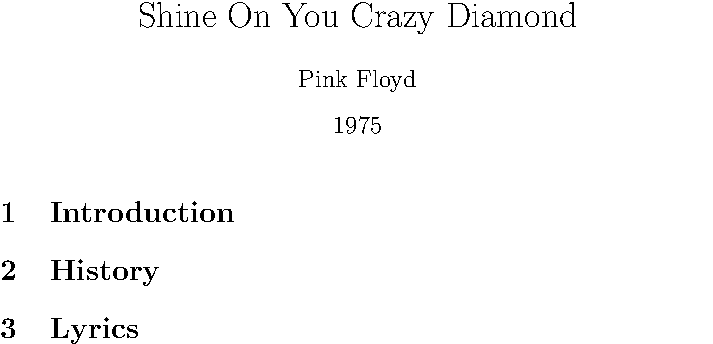
\includegraphics[width=0.8\textwidth]{figures/sections.pdf}
  \end{center}
\end{frame}

\frame[containsverbatim]{
  \frametitle{Sectioning}
  
  \begin{verbatim}
  % For article document class
  \section{...}
  \subsection{...}
  \subsubsection{...}
  \paragraph{...}
  \subparagraph{...}
  
  % Addtionally for book document class
  \chapter{...}
  \end{verbatim}
}

\frame[containsverbatim]{ 
  \frametitle{Text styling}
  
  \begin{LTXexample}
Remember \textbf{when} you \textit{were} young \underline{you} shone \texttt{like} the sun.

{\color{red}Now there's}     {\Huge{a}}       \textbf{\underline{look in} your}          eyes, like     {\tiny{``black holes       {\Large{in the sky}}.''}}
  \end{LTXexample}
}

\frame[containsverbatim]{ 
  \frametitle{Mathematical formulae}
  
  \begin{LTXexample}
\begin{displaymath}
  \lim_{n \to \infty} 
  \sum_{k=1}^n 
  \frac{1}{k^2}
\end{displaymath}

Math $a^2 + b^2 = c^2$ in text style.
  \end{LTXexample}
}

\frame[containsverbatim]{ 
  \frametitle{Chemical formulae}
  
  \begin{LTXexample}
\ce{CO2}

\ce{CO2 + C -> 2 CO}

This is a \ce{H2O} molecule.

I can do charges \ce{CrO4^2-} and much more.
  \end{LTXexample}
}

\frame[containsverbatim]{ 
  \frametitle{Chemical formulae}
  
  \begin{LTXexample}
\chemfig{A*6(-B=C(-CH_3)-D-E-F(=G)=)}
  \end{LTXexample}
}

\frame[containsverbatim]{ 
  \frametitle{Quantities and units}
  
  \begin{LTXexample}
\num{.3e45}

\numlist{10;30;50;70}

\numrange{10}{30}

\si{\kilo\gram\metre\per\square\second}

\SI{1.25}{\metre\per\second}
  \end{LTXexample}
}

\frame[containsverbatim]{ 
  \frametitle{Tables}
  
  \begin{LTXexample}
\begin{tabular}{|l|c|}
  \hline
  Year & Title \\
  \hline
  1973 & The Dark Side of the Moon \\
  1975 & Wish You Were Here \\
  1979 & The Wall \\
  \hline
\end{tabular}
  \end{LTXexample}
}

\frame[containsverbatim]{ 
  \frametitle{Graphics}
  
  \begin{LTXexample}

\includegraphics[scale=0.6]{thewall.png}
  \end{LTXexample}
  
  Note: You can include PDFs! \\
  Note: Graphics remain independent files
}

\frame[containsverbatim]{ 
  \frametitle{Figures and captions}
  
  \begin{LTXexample}
\begin{figure}
  \centering
  
\includegraphics[scale=0.4]{thewall.png}
  \caption{The Wall album cover}
\end{figure}
  \end{LTXexample}
}

\frame[containsverbatim]{ 
  \frametitle{Cross-references}
  
  \begin{LTXexample}
\begin{equation}\label{eq}
E = mc^2
\end{equation}

As shown in Equation \ref{eq}, ...
  \end{LTXexample}
  
  Note: Same approach is used for figures, tables, sections, ...
}

\frame[containsverbatim]{
  \frametitle{Footnotes}
  
  \begin{verbatim}
Remember when you were young, 
  you shone like the sun.

Shine 
on\footnote{Read as if a comma is placed here} 
you crazy 
diamond\footnote{The crazy diamond is Syd Barrett}.

Now there's a look in your eyes, 
  like black holes in the sky.
  \end{verbatim}
}

\begin{frame}
  \frametitle{Footnotes}
  
  \begin{center}
  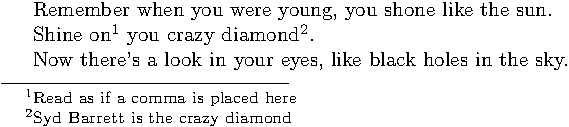
\includegraphics{figures/footnotes.pdf}
  \end{center}
\end{frame}

\frame[containsverbatim]{
  \frametitle{Index}
  
  \begin{verbatim}
\documentclass{article}

\usepackage{makeidx}

\makeindex

\begin{document}

  Shine\index{Sun} on you crazy\newpage
  diamond\index{Diamond}\index{Diamond!Syd}.

  \printindex

\end{document}
  \end{verbatim}
}

\begin{frame}
  \frametitle{Index}
  
  \begin{center}
  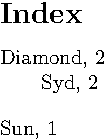
\includegraphics[scale=1.5]{figures/index.pdf}
  \end{center}
\end{frame}

\frame[containsverbatim]{
  \frametitle{Citation}

  \begin{verbatim}
\documentclass{article}

\begin{document}

  Shine on you crazy diamond \cite{pf}.

  \bibliographystyle{plain}
  \bibliography{bibliography.bib}

\end{document}
  \end{verbatim}
}

\begin{frame}
  \frametitle{Reference list}
  
  \begin{center}
  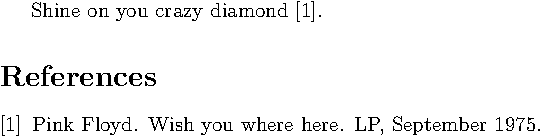
\includegraphics[scale=1]{figures/references.pdf}
  \end{center}
\end{frame}

\frame[containsverbatim]{
  \frametitle{Table of contents, list of figures and tables}
  
  \begin{verbatim}
\documentclass{article}

\begin{document}

  \tableofcontents  % Write out the Table of Contents
  \listoffigures  % Write out the List of Figures
  \listoftables  % Write out the List of Tables

\end{document}
  \end{verbatim}
}

\frame[containsverbatim]{
  \frametitle{Table of contents}
  
  \begin{verbatim}
\documentclass{article}
  
\title{Shine On You Crazy Diamond}
\author{Pink Floyd}
\date{1975}
  
\begin{document}
  \maketitle
  \tableofcontents 
  \section{Introduction}
  Lorem ipsum dolor sit amet, consectetur adipiscing elit.
  \section{History}
  Morbi sagittis enim lorem, a pulvinar orci fringilla ac.
\end{document}
  \end{verbatim}
}

\begin{frame}
  \frametitle{Table of contents}
  
  \begin{center}
  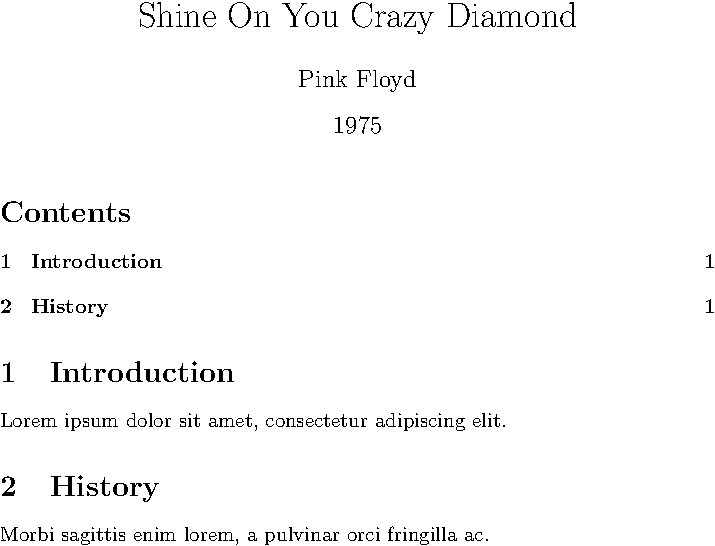
\includegraphics[scale=0.7]{figures/toc.pdf}
  \end{center}
\end{frame}

\frame[containsverbatim]{
  \frametitle{Tracking changes}
  
  \begin{verbatim}
\documentclass{article}

\usepackage{changes}

\definechangesauthor[name={John Doe}, color=blue]{JD}

\begin{document}

  \deleted{...} 
  \replaced{...}{...} 
  \added[id=JD]{...}

\end{document}
  \end{verbatim}
}

\begin{frame}
  \frametitle{Tracking changes}
  
  \begin{center}
  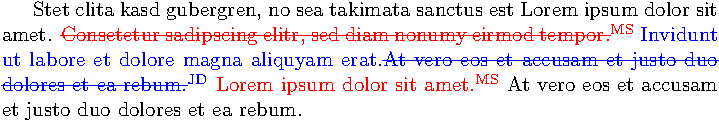
\includegraphics[scale=0.9]{figures/changes.pdf}
  \end{center}
\end{frame}

\begin{frame}
  \frametitle{Reference managers}
  
  \begin{itemize}
  \item References should be managed, using some tool
  \item Many out there, Mendeley, EndNote, RefWorks, ...
  \item Make sure the one you choose supports BibTeX file format
  \item Here we will be using JabRef
  \end{itemize}
\end{frame}

\begin{frame}
  \frametitle{JabRef}
  
  \begin{center}
  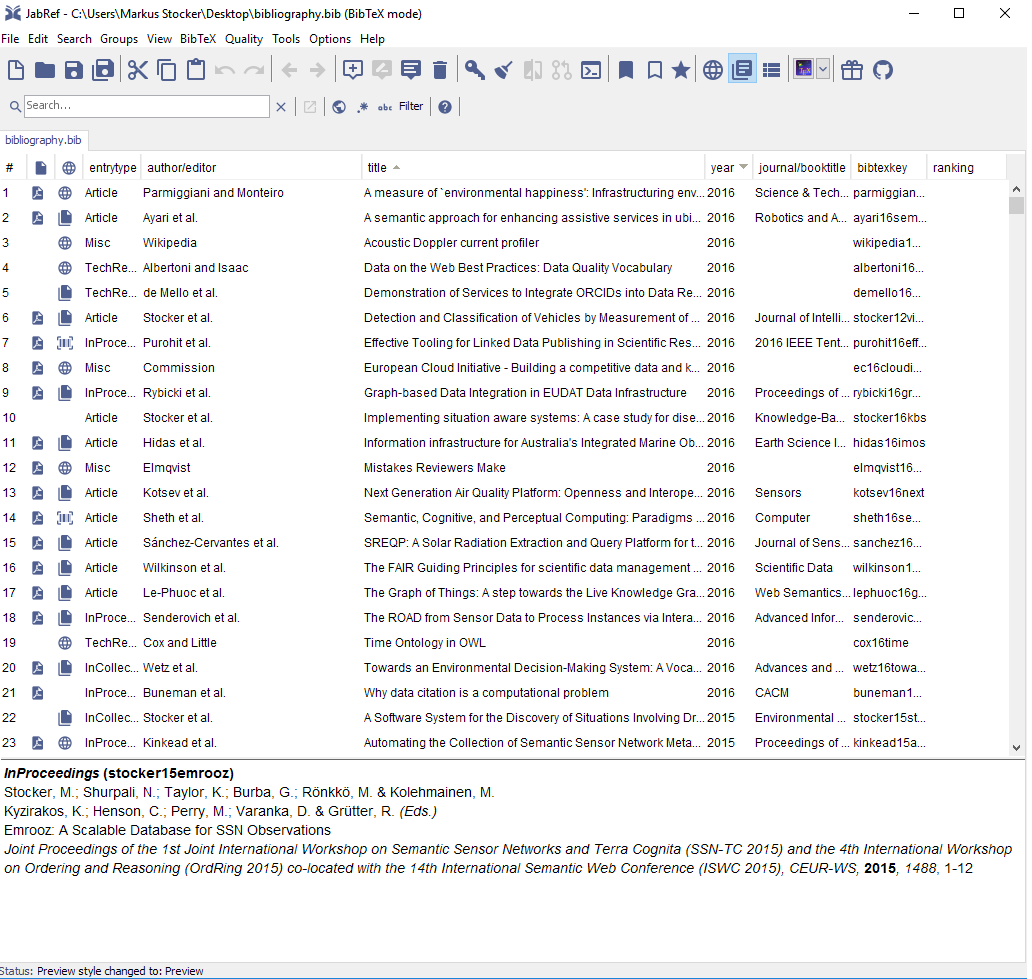
\includegraphics[scale=0.3]{figures/jabref.png}
  \end{center}
\end{frame}

\frame[containsverbatim]{
  \frametitle{BibTeX citation}
  
  \begin{verbatim}
@InProceedings{stocker08sparql,
  title = {{SPARQL Basic Graph Pattern Optimization 
            Using Selectivity Estimation}},
  author = {Stocker, M. and Seaborne, A. 
            and Bernstein, A. and Kiefer, C. 
            and Reynolds, D.},
  booktitle = {Proceeding of the 17th international 
               conference on World Wide Web},
  pages = {595--604},
  year = {2008},
  url = {http://doi.acm.org/10.1145/1367497.1367578},
  doi = {10.1145/1367497.1367578}, 
  publisher = {ACM},
  isbn = {978-1-60558-085-2}
}
  \end{verbatim}
}

\begin{frame}
  \frametitle{Obtain citations}
  
  \begin{center}
  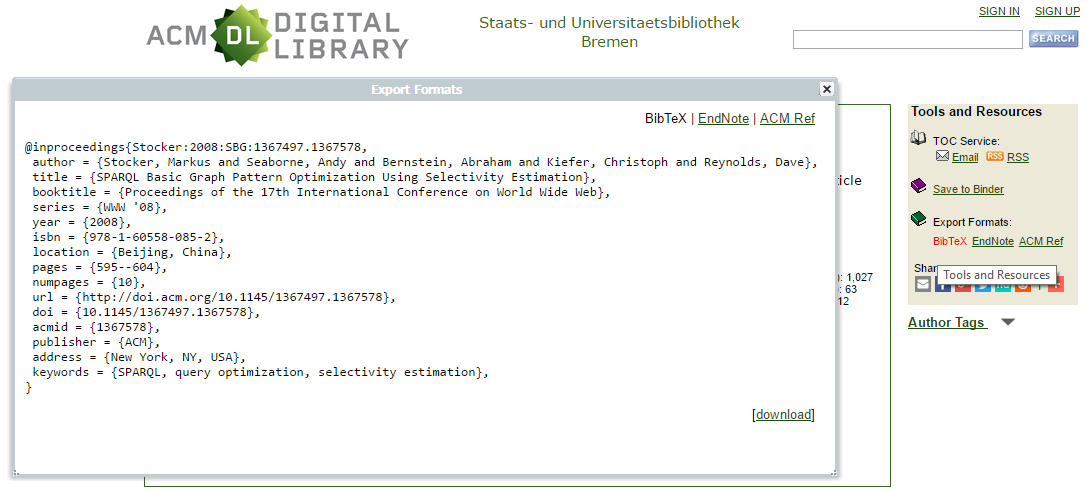
\includegraphics[scale=0.4]{figures/acm-citation.png}
  \end{center}
\end{frame}

\frame[containsverbatim]{
  \frametitle{Cite}

  \begin{verbatim}
\documentclass{article}

\begin{document}

  In \cite{stocker08sparql}, the authors show that ...

  \bibliographystyle{plain}
  \bibliography{bibliography.bib}

\end{document}
  \end{verbatim}
}


\begin{frame}
  \frametitle{Journal templates}
  
  \begin{itemize}
    \item \LaTeX~is pretty much the standard in publishing
    \item Most journal provide \LaTeX~templates
    \item In fact, they are typically by the publisher
    \item Selected publishers with \LaTeX~instructions
    \begin{itemize}
      \item Elsevier, Springer, IOS Press, PLOS, Taylor \& Francis, Wiley, SAGE, IEEE, MDPI, Nature Publishing Group, ...
    \end{itemize}
    \item Simply search for "[PUBLISHER/JOURNAL] latex template"
  \end{itemize}
\end{frame}

\begin{frame}
  \frametitle{Elsevier \LaTeX~instructions}
  
  \begin{center}
    
\includegraphics[width=0.9\textwidth]{figures/elsevier.png}
  \end{center}
\end{frame}

\begin{frame}
  \frametitle{Elsarticle \LaTeX~document class}
  
  \begin{center}
    
\includegraphics[height=0.8\textheight]{figures/elsarticle.png}
  \end{center}
\end{frame}

\begin{frame}
  \frametitle{\LaTeX~for slides}
  
  \begin{itemize}
    \item \LaTeX~can be used to create slides
    \item In fact, these slides were done with \LaTeX
    \item Obviously, for a \LaTeX~course!
    \item Widely used document class is called \texttt{beamer}
  \end{itemize}
\end{frame}


\frame[containsverbatim]{
  \frametitle{Slides with \texttt{beamer} document class}
  
  \begin{verbatim}
\documentclass{beamer}

\begin{document}

  \begin{frame}
    \frametitle{Outline}

    \begin{itemize}
      \item ...
    \end{itemize}
  \end{frame}

\end{document}
  \end{verbatim}
}

\begin{frame}
  \frametitle{\LaTeX~for posters}
  
  \begin{itemize}
    \item There are many document classes for posters
    \item a0poster, baposter, sciposter, beamerposter, tikzposter, Jacobs, ...
    \item As for slides, whether you use \LaTeX~for posters depends
    \begin{itemize}
      \item Is there a corresponding \LaTeX~article?
      \item Are you reusing content from the article in the poster?
      \item Especially formulae, references, etc.
    \end{itemize}
    \item Slides as PDF, not as PPTX (obviously)
  \end{itemize}
\end{frame}

\begin{frame}
  \frametitle{Jacobs poster}
  
  \begin{center}
    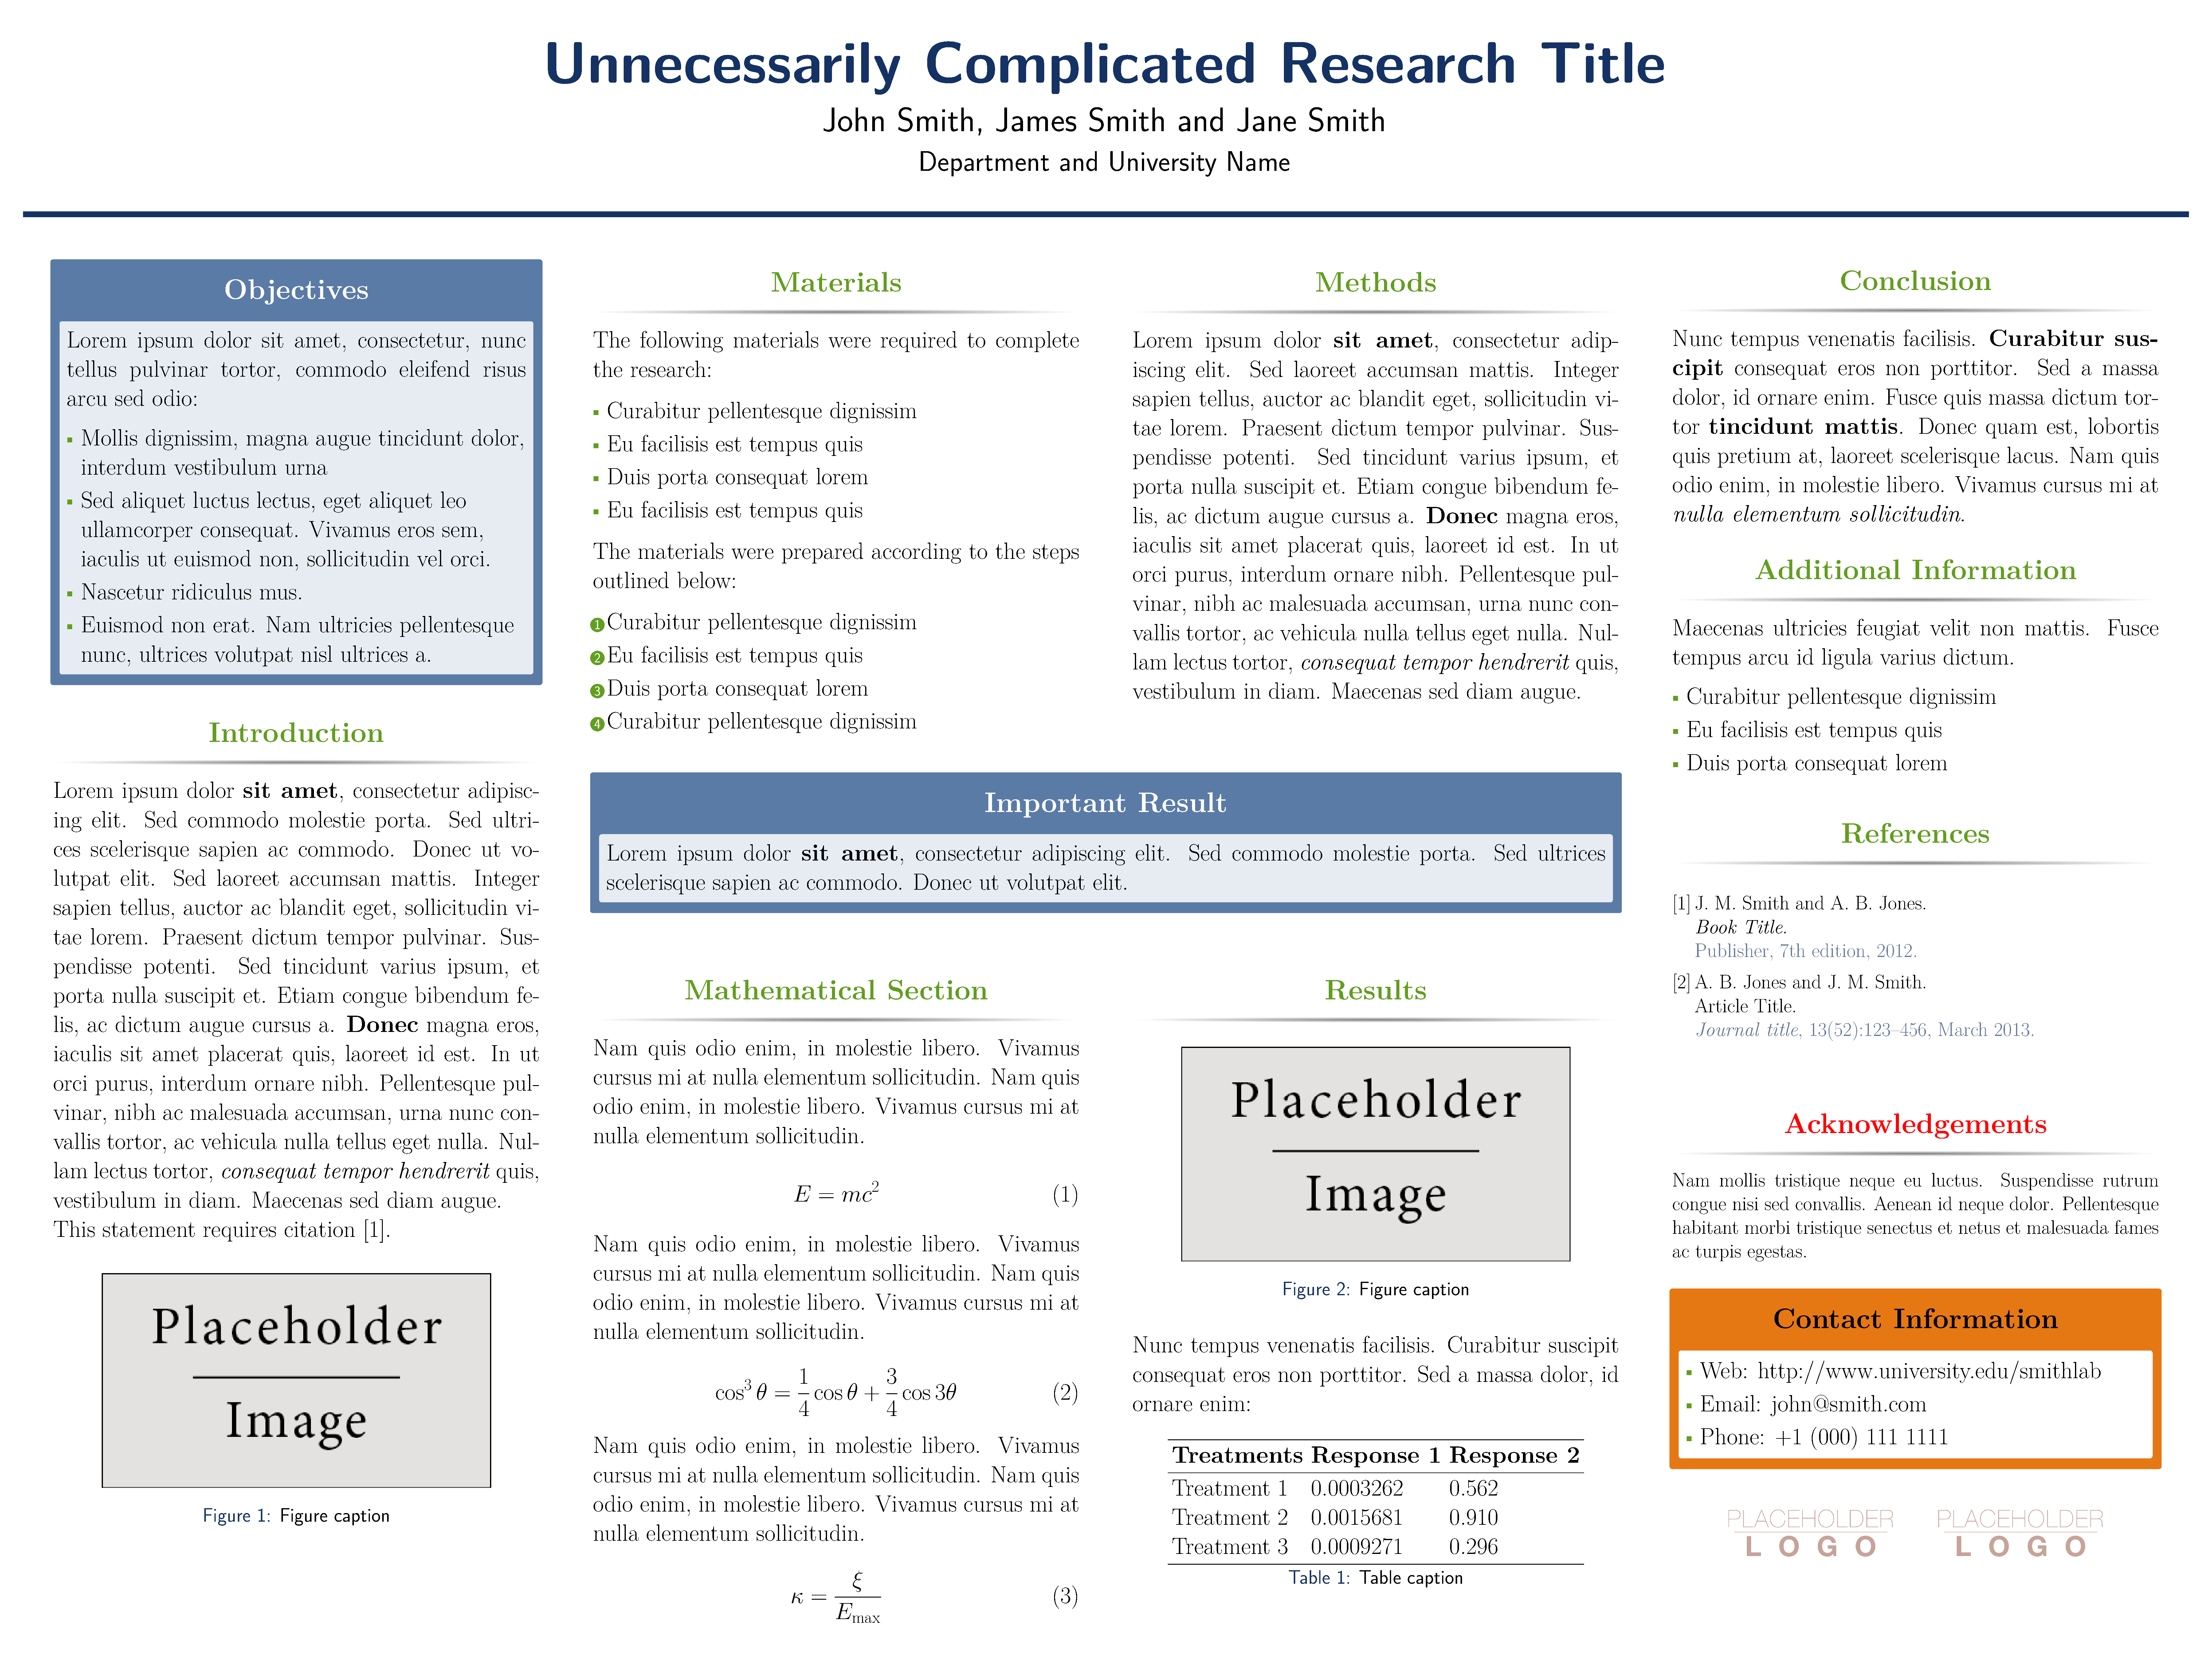
\includegraphics[height=0.8\textheight]{figures/poster.pdf}
  \end{center}
\end{frame}

\begin{frame}
  \frametitle{\LaTeX~for ...}
  
  \begin{itemize}
    \item You can use \LaTeX~for a lot of things!
    \item Plenty of document classes and packages
    \item For instance, my CV is written in \LaTeX
    \item \LaTeX~can create graphics, not just include them
    \item You can write music with \LaTeX
  \end{itemize}
\end{frame}

\frame[containsverbatim]{
  \frametitle{Write music with \LaTeX}
  
  \begin{verbatim}
\documentclass{article}

\begin{document}

  \begin{lilypond}
    \relative c' {
      c2 g'2 \times 2/3 { f8 e d } c'2 g4
    }
  \end{lilypond}

\end{document}
  \end{verbatim}
}

\begin{frame}
  \frametitle{Write music with \LaTeX}
  
  \begin{center}
    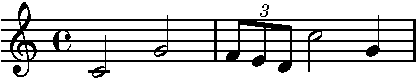
\includegraphics{figures/music.pdf}
  \end{center}
  
  \vspace{1cm}
  
  \begin{center}
    \url{https://martin-thoma.com/how-to-write-music-with-latex/}
  \end{center}
\end{frame}

\begin{frame}
  \frametitle{Some thoughts on collaborative writing}
  
  \begin{itemize}
    \item Typically, we work collaboratively on articles
    \item Collaborative writing is not entirely trivial
    \item Too often we send around files by email
    \item Google Docs has eased this considerably
    \item It is super convenient, also for editing
    \item However, not for complex documents
    \item Write locally and safe in Dropbox is also popular
    \item But Dropbox doesn't merge changes
  \end{itemize}
\end{frame}

\begin{frame}
  \frametitle{Online \LaTeX}
  
  \begin{itemize}
    \item There exist a number of online platforms
    \item For instance Overleaf and ShareLaTeX
    \item Overleaf is an online \LaTeX~collaborative writing tool
    \item With a reasonable free plan
    \item How to work offline, e.g. on an airplane?
  \end{itemize}
  
  \vspace{1cm}
  
  \begin{flushright}
    \url{https://www.overleaf.com/}
  \end{flushright}
\end{frame}

\begin{frame}
  \frametitle{Overleaf}
  
  \begin{center}
    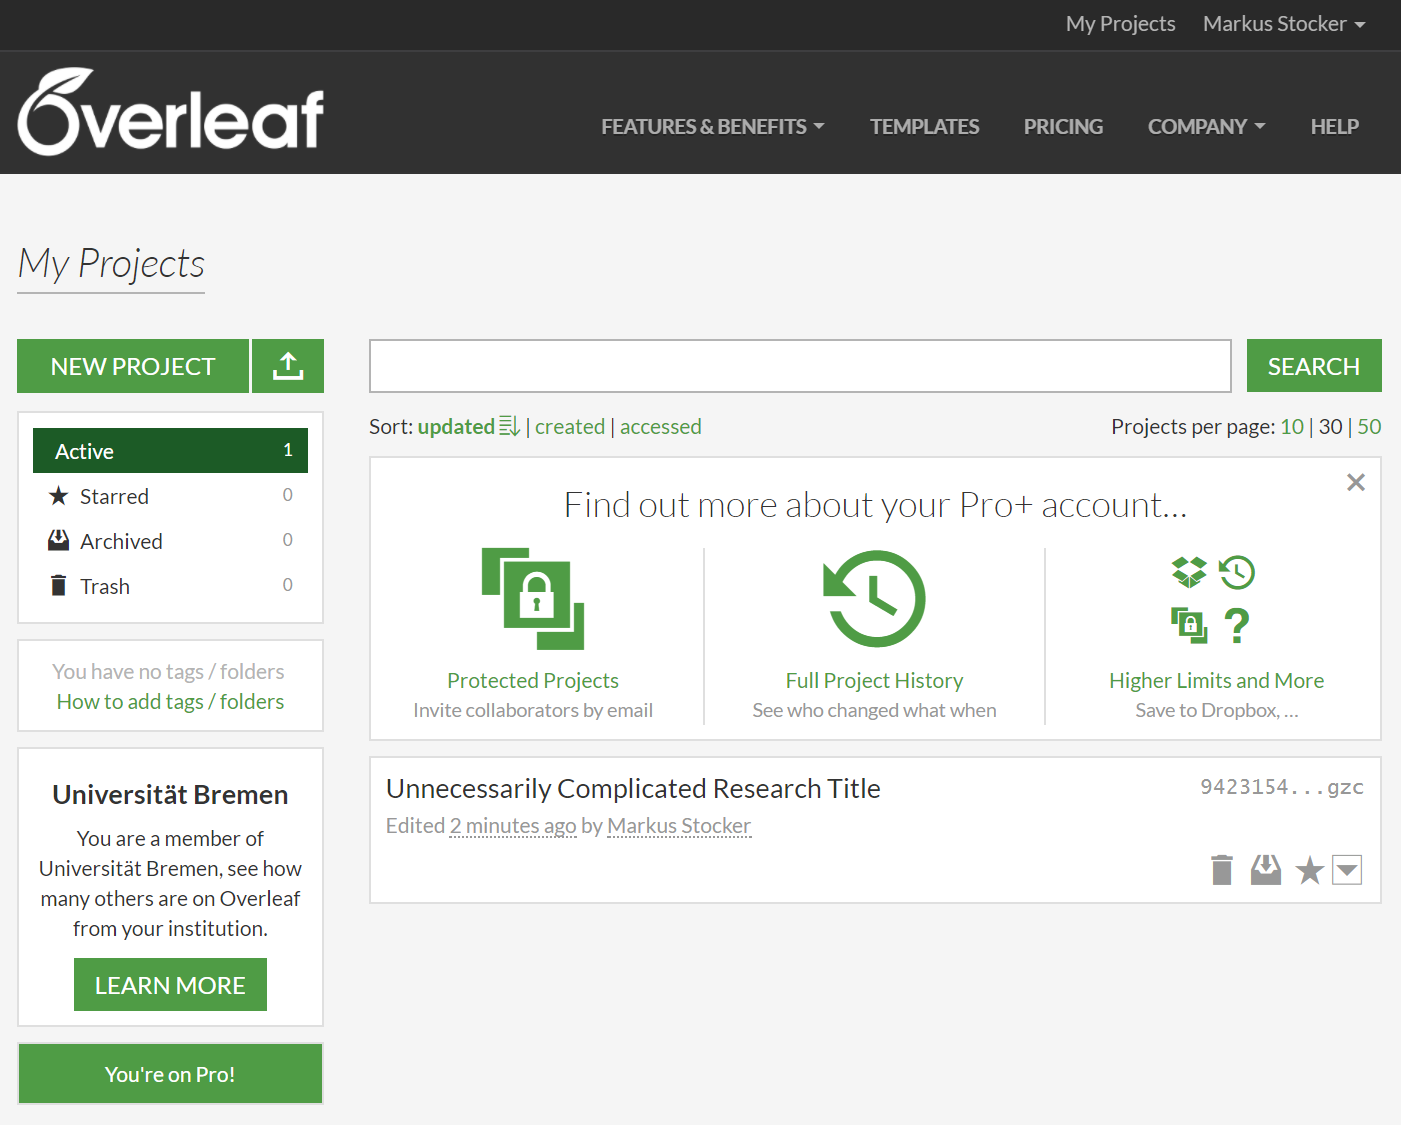
\includegraphics[height=0.8\textheight]{figures/overleaf-1.png}
  \end{center}
\end{frame}

\begin{frame}
  \frametitle{Overleaf}
  
  \begin{center}
    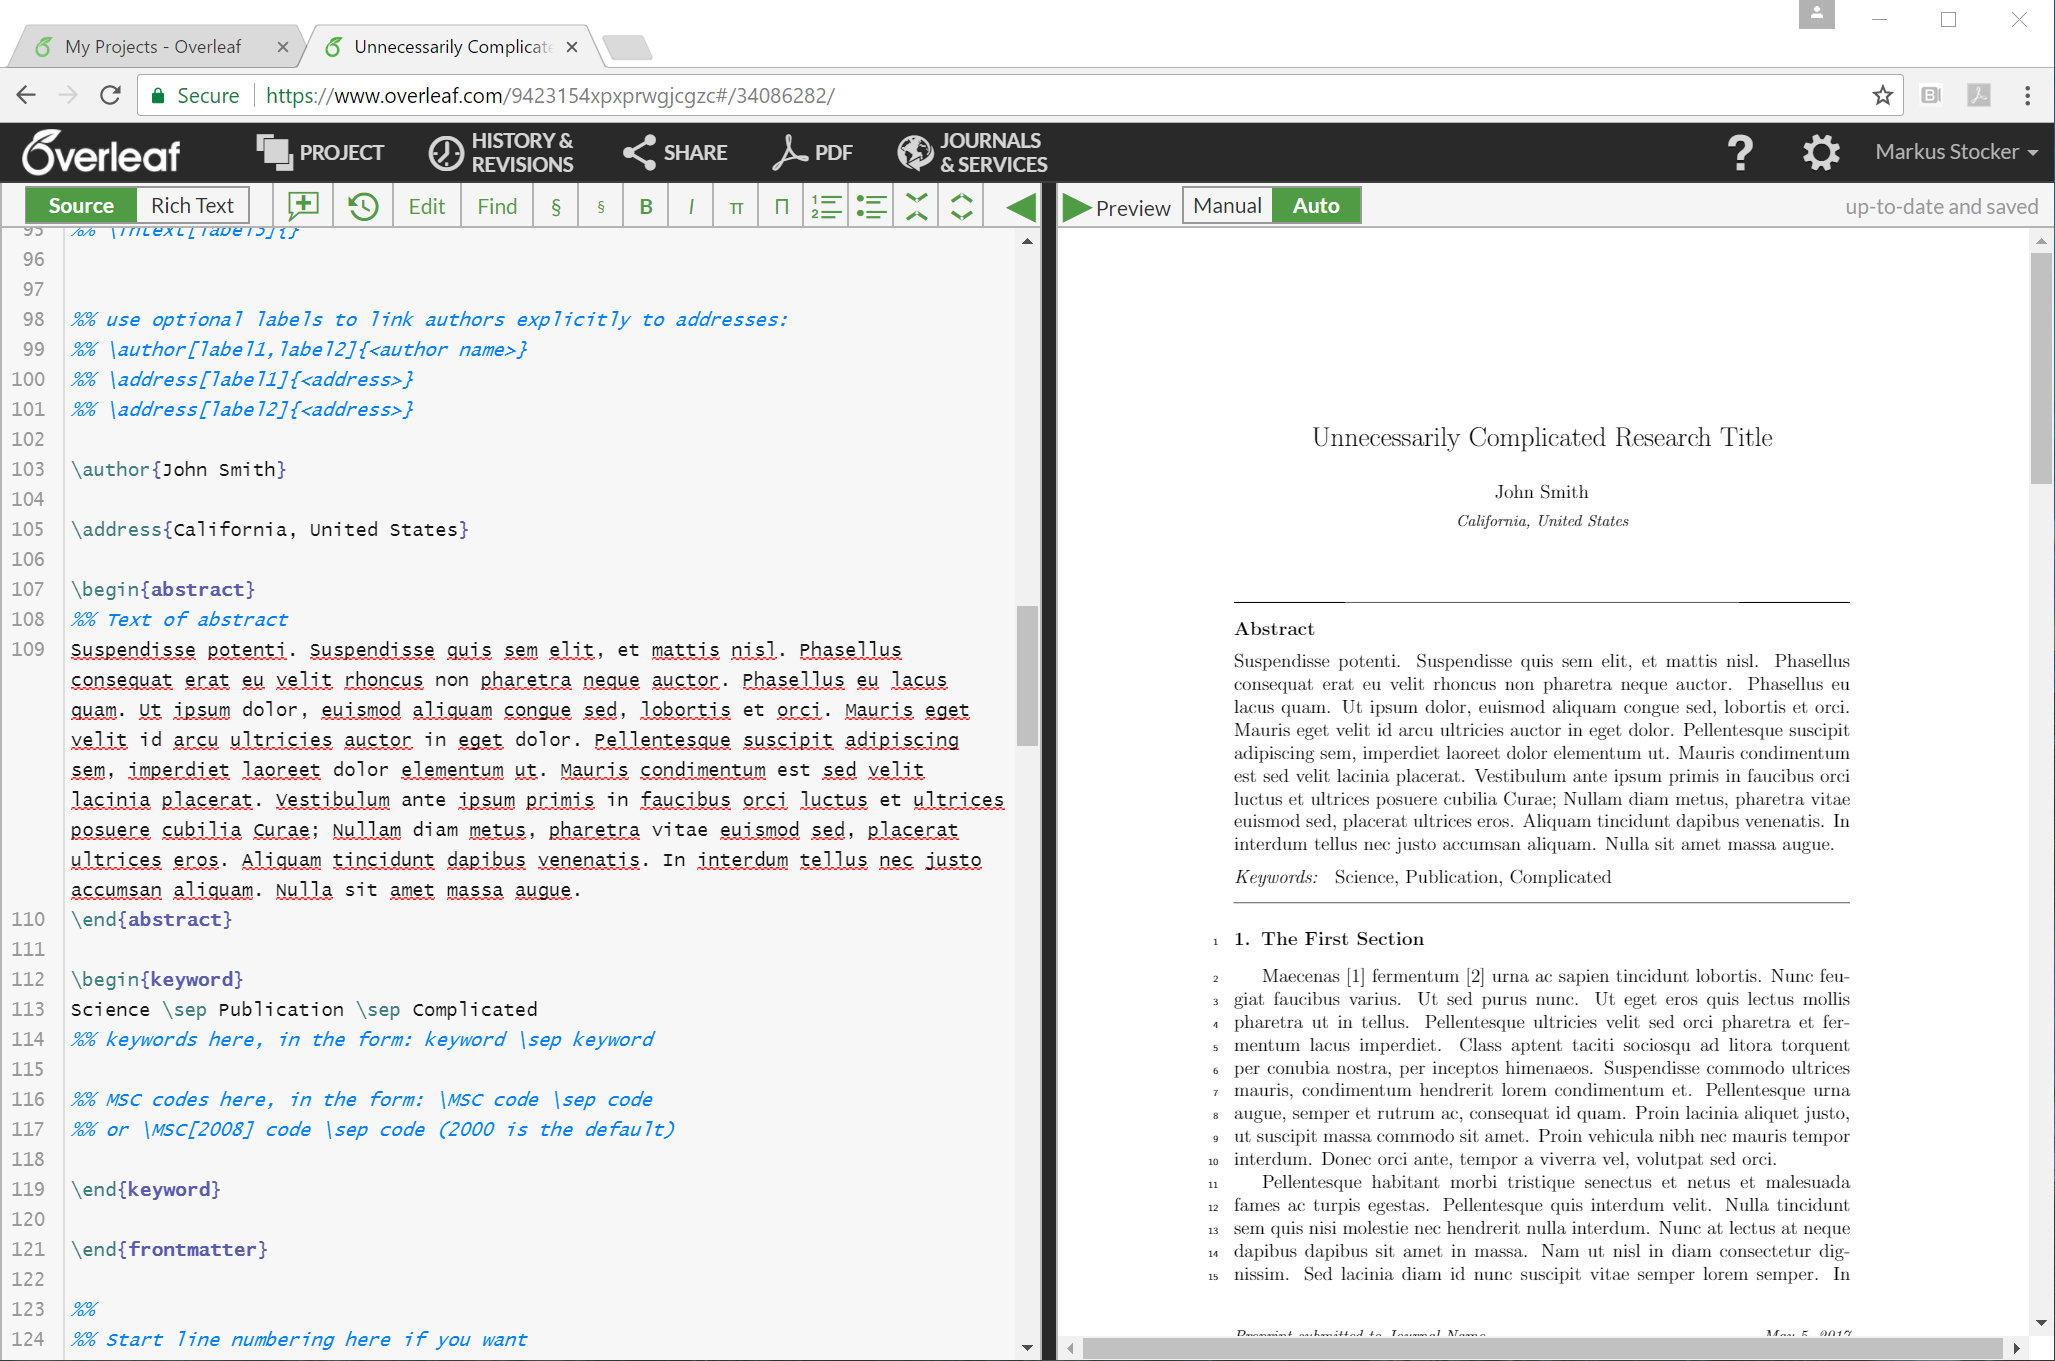
\includegraphics[height=0.8\textheight]{figures/overleaf-2.png}
  \end{center}
\end{frame}

\begin{frame}
  \frametitle{Git}
  
  \begin{itemize}
    \item One of many version control systems
    \item Supports tracking changes and coordinating work on files
    \item Primarily used for software development
    \item Great for collaborative writing with \LaTeX
    \item Choose an online Git repository, e.g. GitHub, Bitbucket
    \item Working against online repository 
    \begin{itemize}
      \item Enables collaborative writing
      \item Ensures you have a backup
      \item Facilitates work at the office, home, coffee shop, ...
    \end{itemize}
    \item Very powerful approach
    \item As for \LaTeX, basics are relatively easy, details more intricate
  \end{itemize}
\end{frame}


\begin{frame}
  \frametitle{Git}
  
  \begin{center}
    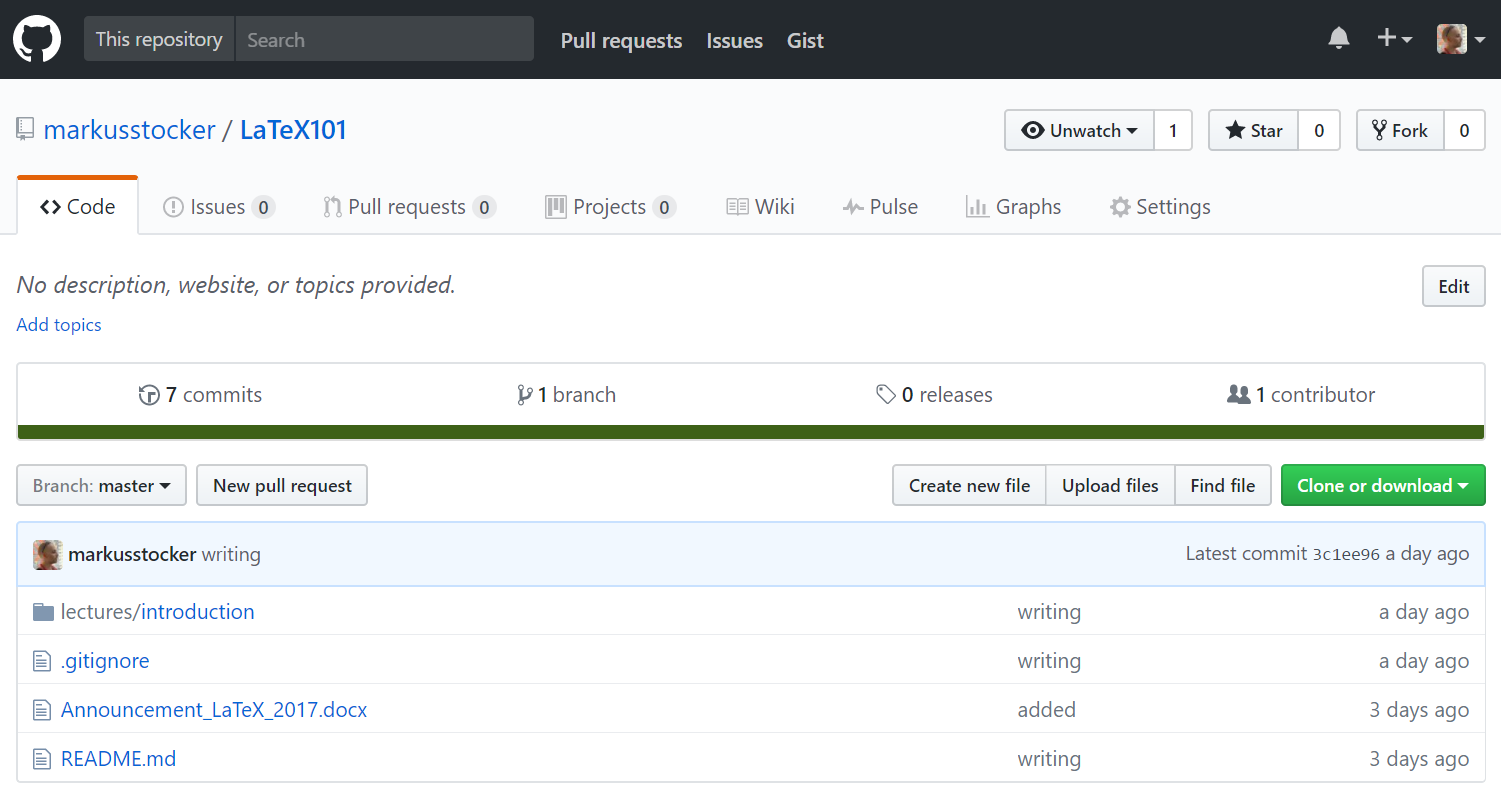
\includegraphics[width=0.8\textwidth]{figures/git.png}
  \end{center}
  
  \begin{flushright}
    \url{https://github.com/markusstocker/LaTeX101}
  \end{flushright}
\end{frame}

\begin{frame}
  \frametitle{Basic Git commands}
  
  \begin{itemize}
    \item \texttt{git clone}: Clone remote repository in local environment
    \item \texttt{git status}: Check what has changed
    \item \texttt{git add}: Add files to the local repository
    \item \texttt{git commit}: Record changes to local repository
    \item \texttt{git push}: Push changes to remote repository
    \item \texttt{git pull}: Fetch changes from remote repositorys
  \end{itemize}
\end{frame}

\begin{frame}
  \frametitle{Take aways}
  
  \begin{itemize}
    \item You need time to learn \LaTeX~and other presented tools
    \item Practice, the basics are relatively straightforward
    \item The optimal approach ultimately depends on your needs
    \item Needs are typically different between projects
    \item For most problems there is an answer online
  \end{itemize}
\end{frame}

\end{document}

% TODO: Describe JabRef
% Resources
% - https://tobi.oetiker.ch/lshort/lshort.pdf
% - https://de.sharelatex.com/learn/Chemistry_formulae
